\chapter{单模光态：数态、相干态、热态、压缩态}
\label{chap:e06}

\begin{chapteropening}
上一章我们做成了一件大事：把整个电磁场拆成一堆模式，并证明\emph{每一个模式在数学上就是一个谐振子}——于是"光子"有了精确定义，它是某个模式的一次激发。可是同一个模式，就像同一个弹簧，可以处在千姿百态的量子态里。本章要回答的问题很朴素，也很关键：\textbf{在同一个模式里，光到底能装成哪几种样子？它们看起来有什么不同？}我们会发现，光子数是否钉死、相位是否稳定、强度是否涨落，会让四种典型光态——数态、相干态、热态、压缩态——即使平均光子数一模一样，也留下截然不同的"点击统计指纹"。为了把这四种光一次量到底，我们先造一把统一的尺子：\emph{零延迟成对因子} \(b_2\)。然后对每一种光，我们都手把手把它的 \(b_2\) 算出来——数态给 \(1-1/n\)（反聚束），相干态给 \(1\)（泊松基线），热态给 \(2\)（聚束）。这个"多出来的一倍"，正是后面强度干涉（Hanbury Brown--Twiss）赖以工作的种子。
\end{chapteropening}

\section{一把统一的尺子：零延迟成对因子}
\label{sec:e06-b2}

先想清楚我们到底要量什么。第 \ref{chap:e05} 章已经知道，望远镜每次"点击"背后站着一个湮灭算符 \(\hat a\)：某个模式里少了一个光子。如果我们盯住同一个模式，问"两个点击几乎同时到来的倾向有多强"，这就是光态最本质的区别之一——它不体现在平均有多亮，而体现在\emph{光子爱不爱扎堆}。

平均光子数谁都会算，就是数算符的期望 \(\langle\hat n\rangle\)。可只看平均，数态、相干态、热态可以完全一样（都调到 \(\langle\hat n\rangle=\bar n\)），却是三种截然不同的光。真正把它们分开的，是"成对"这件事：在同一个模式里，能凑出多少对光子？

\paragraph{为什么用阶乘矩，而不是平方}
\label{sec:e06-why-factorial}

一个初学者最自然的想法是用 \(\langle\hat n^2\rangle\) 来衡量"成对"。这恰恰是本节要纠正的第一个坑。设想模式里此刻有 \(N\) 个光子，我们要数"能从中挑出多少个\emph{有序光子对}"。挑第一个光子有 \(N\) 种选法，挑第二个——它必须是\emph{另一个}光子，不能是刚才那一个——只剩 \(N-1\) 种选法。所以有序对的数目是
\[
  N\times(N-1)=N(N-1),
\]
而不是 \(N\times N=N^2\)。两者相差的那一项 \(N^2-N(N-1)=N\)，正是"让同一个光子和它自己配对"的假项。物理上，\textbf{同一个光子不能和自己配成一对}：探测器吸收掉它一次，它就没了，不可能再被第二个探测器同时吸收。所以凡是涉及"两个点击"的量，正确的计数一定是 \(N(N-1)\)，即所谓的\emph{二阶阶乘矩}（second factorial moment）。这个"自配对要扣掉"的道理，会在第 \ref{chap:e07} 章讲光电探测的正规序（normal ordering）时再从算符层面证一遍；这里我们先从"数对子"的组合意义上把它认下来。

于是我们定义零延迟成对因子（zero-delay pair factor）：
\begin{equation}
  b_2\equiv\frac{\langle\hat n(\hat n-1)\rangle}{\langle\hat n\rangle^{2}} .
  \label{eq:e06-b2def}
\end{equation}
\begin{formulaexplain}
分子 \(\langle\hat n(\hat n-1)\rangle\) 是"平均能凑出多少对光子"（扣掉了自配对）；分母 \(\langle\hat n\rangle^2\) 是"若光子彼此独立、随机到达时应有的对数基线"。\(b_2\) 就是二者之比：光子扎堆的倾向相对随机基线放大了多少倍。
\end{formulaexplain}

逐个交代记号。\(\hat n=\hat a^\dagger\hat a\) 是数算符，本征值 \(N=0,1,2,\dots\) 是纯整数、无单位；\(\langle\cdot\rangle\) 是对光态求期望（纯态取内积，混合态取迹 \(\operatorname{Tr}(\rho\,\cdot)\)）。分子 \(\langle\hat n(\hat n-1)\rangle\) 无单位，是"平均对数"；分母 \(\langle\hat n\rangle^2\) 也无单位。所以 \(b_2\) 是一个纯数，它不关心这个模式有多亮（分母已经把亮度归一化掉了），只关心\emph{光子在同一模式里成对到来的倾向，相对于"各自独立、互不通气"的随机基线，是多还是少}。

为什么"独立随机"给出的基线恰好让分子约等于分母？下一节算相干态时会严格验证。这里先把三条判据摆出来，它是本章后面反复对照的标尺：
\begin{itemize}
  \item \(b_2=1\)：\textbf{独立泊松基线}。光子各来各的、互不通气，看到一个不改变马上再看到一个的概率。
  \item \(b_2>1\)：\textbf{聚束}（bunching）。光子爱扎堆，"要来一起来"，成对概率高于随机基线——热光就是如此。
  \item \(b_2<1\)：\textbf{反聚束}（antibunching），也叫\emph{亚泊松}。光子相互回避，"来了一个就不容易马上来第二个"，成对概率低于随机基线——这是纯量子效应，经典波做不到。
\end{itemize}

有了这把尺子，我们就逐一"量"四种光。策略始终一样：先写出该态的光子数分布 \(P(N)\)（或密度矩阵），算出 \(\langle\hat n\rangle\) 和 \(\langle\hat n(\hat n-1)\rangle\)，代进式 \eqref{eq:e06-b2def}。每一步都不跳。

\section{数态：光子数钉死的光}
\label{sec:e06-fock}

从最"干脆"的光开始。第 \ref{chap:e05} 章已经见过数态（number state）\(|n\rangle\)，又叫 Fock 态：它是数算符的本征态，\(\hat n|n\rangle=n|n\rangle\)，意思是这个模式里\emph{恰好}有 \(n\) 个光子，一个不多、一个不少、没有任何涨落。它的计数分布是一根孤零零的竖线：
\begin{equation}
  P(N)=\delta_{Nn}=
  \begin{cases}
    1, & N=n,\\
    0, & N\neq n.
  \end{cases}
  \label{eq:e06-fock-dist}
\end{equation}
\begin{formulaexplain}
\(P(N)\) 是"数到 \(N\) 个光子"的概率；\(\delta_{Nn}\) 是克罗内克符号（Kronecker delta），只有 \(N=n\) 时为 1、其余为 0。它说明数态测量光子数永远得到同一个值 \(n\)，毫无起伏。
\end{formulaexplain}

正因为 \(P(N)\) 只在 \(N=n\) 处非零，所有期望都退化成"直接代入 \(N=n\)"。平均光子数是
\[
  \langle\hat n\rangle=\sum_{N}N\,P(N)=n\cdot 1=n,
\]
二阶阶乘矩同样只留下 \(N=n\) 一项：
\[
  \langle\hat n(\hat n-1)\rangle=\sum_{N}N(N-1)\,P(N)=n(n-1).
\]
代进成对因子的定义 \eqref{eq:e06-b2def}：
\begin{equation}
  b_{2,\text{Fock}}=\frac{n(n-1)}{n^{2}}=\frac{n-1}{n}=1-\frac{1}{n}.
  \label{eq:e06-fock-b2}
\end{equation}
\begin{formulaexplain}
数态的成对因子只差随机基线 \(1\) 一个 \(1/n\)。光子数越少，反聚束越明显；\(n=1\) 时 \(b_2\) 一路压到 \(0\)。
\end{formulaexplain}

这条结果值得咀嚼。对任意有限 \(n\)，都有 \(b_2=1-1/n<1\)：数态总是\emph{反聚束}的。原因一目了然——模式里只有 \(n\) 个光子，用掉一个数对子就少一个"库存"，所以能凑的对数 \(n(n-1)\) 天然比"独立随机"的 \(n^2\) 少。特别地，取单光子态 \(n=1\)：
\[
  b_{2,\text{Fock}}(n=1)=1-\frac{1}{1}=0.
\]
这是反聚束的\emph{理想极限}。物理意义斩钉截铁：一个模式里只有一个光子，它被吸收一次就没了，绝不可能让两个探测器\emph{同时}各收到一个——所以"成对"概率精确为零。这正是单光子源（single-photon source）最珍贵的量子签名，实验室里的共振荧光可以清楚地做出 \(b_2\to 0\) \citep{1977PhRvL..39..691K}。

不过要提醒：天体光几乎从不以纯数态到达。源区里无数独立发射体、漫长的传播路径、望远镜和探测器都会把未观测的自由度混进来，把 \(b_2\) 从 \(0\) 一路拉回接近 \(1\)。数态在这里的价值，是给我们一个\emph{下限锚点}和一句提醒：点击统计测的是光子数的关联，而不是一条连续波形。当 \(n\to\infty\) 时 \(b_2\to 1\)，反聚束消失——光子一多，量子的"独占性"就淹没在数量里，这也预告了为什么明亮天体很难显出非经典统计。

\section{相干态：最像经典激光的光}
\label{sec:e06-coherent}

第 \ref{chap:e04} 章末尾预告过一种"最接近经典振动"的量子态；现在正式请它出场。相干态（coherent state）\(|\alpha\rangle\) 定义为湮灭算符的本征态：
\begin{equation}
  \hat a\,|\alpha\rangle=\alpha\,|\alpha\rangle,
  \qquad
  \bar n\equiv\langle\hat n\rangle=|\alpha|^{2}.
  \label{eq:e06-coherent-def}
\end{equation}
\begin{formulaexplain}
\(|\alpha\rangle\) 满足"被湮灭算符作用后自己不变、只乘一个复数 \(\alpha\)"。\(\alpha\) 是无量纲复振幅：它的模平方 \(|\alpha|^2\) 给平均光子数 \(\bar n\)，辐角 \(\arg\alpha\) 给相位。这是一支相位稳定、振幅确定的"经典波"的量子版本。
\end{formulaexplain}

先解释这个定义为什么"经典"。\(\alpha\) 是一个无量纲的复数，可以把它想成第 \ref{chap:e01} 章那支"旋转的箭头"（复振幅）：模长 \(|\alpha|\) 是振幅，辐角是相位，两者都确定，没有相位抖动——这正是理想激光的图像。稳定实验室激光在很多测量里都极接近相干态 \citep{1963PhRv..131.2766G}。而"\(\hat a|\alpha\rangle=\alpha|\alpha\rangle\)"这条奇特性质意味着：\emph{从相干态里拿走一个光子，它还是同一个相干态}——就像从一片浩瀚的相位一致的波里舀走一滴，波纹丝毫不改。这是它区别于数态的根本。

\paragraph{从定义推出泊松分布}
\label{sec:e06-coherent-poisson}

第 \ref{chap:e04} 章两次预告过"相干态的光子数服从泊松分布"，这里我们把它\emph{从定义推出来}，而不是空降。唯一的原料就是本征方程 \eqref{eq:e06-coherent-def}，加上第 \ref{chap:e05} 章的湮灭算符作用规则 \(\hat a|N\rangle=\sqrt{N}\,|N-1\rangle\)。

\textbf{第一步：把相干态写成数态的叠加。}数态 \(\{|N\rangle\}\) 是这个模式的完备基底，所以任何单模态都能展开成它们的线性组合。设
\[
  |\alpha\rangle=\sum_{N=0}^{\infty}c_N\,|N\rangle,
\]
其中待定系数 \(c_N=\langle N|\alpha\rangle\) 就是"这个态里含 \(N\) 光子成分"的振幅。把它代进本征方程左边，用 \(\hat a|N\rangle=\sqrt{N}\,|N-1\rangle\)（注意 \(N=0\) 项被湮灭掉、不贡献）：
\[
  \hat a\,|\alpha\rangle
  =\sum_{N=1}^{\infty}c_N\sqrt{N}\,|N-1\rangle
  =\sum_{M=0}^{\infty}c_{M+1}\sqrt{M+1}\,|M\rangle,
\]
最后一步令 \(M\equiv N-1\) 重新编号。而本征方程右边是
\[
  \alpha\,|\alpha\rangle=\sum_{M=0}^{\infty}\alpha\,c_M\,|M\rangle.
\]
\textbf{第二步：逐个数态比对系数，得到递推。}两边都是数态基底上的展开，对应系数必须相等，于是对每个 \(M\)：
\[
  c_{M+1}\sqrt{M+1}=\alpha\,c_M
  \quad\Longrightarrow\quad
  c_{M+1}=\frac{\alpha}{\sqrt{M+1}}\,c_M .
\]
\textbf{第三步：解递推。}从 \(c_0\) 出发逐级往上爬，每加一个光子就乘一个 \(\alpha/\sqrt{N}\)：
\[
  c_1=\frac{\alpha}{\sqrt1}c_0,\quad
  c_2=\frac{\alpha}{\sqrt2}c_1=\frac{\alpha^2}{\sqrt{2!}}c_0,\quad\dots\quad
  c_N=\frac{\alpha^{\,N}}{\sqrt{N!}}\,c_0 .
\]
\textbf{第四步：归一化定出 \(c_0\)。}要求 \(\langle\alpha|\alpha\rangle=\sum_N|c_N|^2=1\)。把上式代入，并点名使用指数级数 \(\sum_{N}x^N/N!=e^{x}\)（这里 \(x=|\alpha|^2\)）：
\[
  \sum_{N=0}^{\infty}|c_N|^2
  =|c_0|^2\sum_{N=0}^{\infty}\frac{|\alpha|^{2N}}{N!}
  =|c_0|^2\,e^{|\alpha|^2}=1
  \quad\Longrightarrow\quad
  |c_0|^2=e^{-|\alpha|^2}.
\]
取正实的 \(c_0=e^{-|\alpha|^2/2}\)（相位可任选，不影响概率）。至此相干态的数态展开就完全确定了。\textbf{第五步：读出光子数概率。}数到 \(N\) 个光子的概率正是该分量振幅的模平方：
\begin{equation}
  P(N)=\big|\langle N|\alpha\rangle\big|^2=|c_N|^2
  =\frac{|\alpha|^{2N}}{N!}\,e^{-|\alpha|^2}
  =e^{-\bar n}\,\frac{\bar n^{\,N}}{N!},
  \qquad N=0,1,2,\dots
  \label{eq:e06-poisson}
\end{equation}
\begin{formulaexplain}
\(P(N)\) 是数到 \(N\) 个光子的概率；\(\bar n=|\alpha|^2\) 是平均光子数；\(N!\) 是离散计数的归一化。它由本征方程一路推出，正是第 \ref{chap:e03} 章那条"独立随机到达"的泊松分布——相干态的光子彼此独立，各来各的。
\end{formulaexplain}

最后一步用了 \(\bar n=|\alpha|^2\)，把复振幅换成了平均光子数。式 \eqref{eq:e06-poisson} 就是\textbf{泊松分布}（Poisson distribution），它不是被断言的，而是从"\(\hat a|\alpha\rangle=\alpha|\alpha\rangle\)"一步步逼出来的：本征方程给递推，递推给系数，归一化定常数，模平方给概率。这里 \(\bar n=|\alpha|^2\) 无单位，\(N!\) 是 \(N\) 的阶乘。式 \eqref{eq:e06-poisson} 与第 \ref{chap:e03} 章讲散粒噪声时那条泊松分布\emph{完全同形}——这不是巧合：相干态的光子是彼此独立的随机事件，正是散粒噪声（shot noise）的来源，方差等于均值 \(\operatorname{Var}(N)=\bar n\)。

\paragraph{手把手算相干态的成对因子}
\label{sec:e06-coherent-b2}

现在用尺子量它。要算 \(b_2\)，我们需要二阶阶乘矩 \(\langle N(N-1)\rangle\)。把泊松分布 \eqref{eq:e06-poisson} 代进求和，一步不省：
\[
  \langle N(N-1)\rangle
  =\sum_{N=0}^{\infty}N(N-1)\,e^{-\bar n}\frac{\bar n^{\,N}}{N!}.
\]
\textbf{第一步：砍掉为零的项。}求和的每一项都带因子 \(N(N-1)\)。当 \(N=0\) 时 \(N(N-1)=0\)；当 \(N=1\) 时 \(N(N-1)=1\cdot 0=0\)。所以 \(N=0\) 和 \(N=1\) 两项对求和\emph{毫无贡献}，可以直接从 \(N=2\) 起加：
\[
  \langle N(N-1)\rangle
  =\sum_{N=2}^{\infty}N(N-1)\,e^{-\bar n}\frac{\bar n^{\,N}}{N!}.
\]
\textbf{第二步：约掉阶乘。}注意阶乘的定义 \(N!=N(N-1)(N-2)!\)，所以 \(N(N-1)/N!=1/(N-2)!\)。这一步把碍事的 \(N(N-1)\) 干净地消掉：
\[
  \langle N(N-1)\rangle
  =e^{-\bar n}\sum_{N=2}^{\infty}\frac{\bar n^{\,N}}{(N-2)!}.
\]
\textbf{第三步：换元求和。}令 \(m\equiv N-2\)（于是 \(N=2\) 对应 \(m=0\)，\(N\to\infty\) 对应 \(m\to\infty\)），并把 \(\bar n^{\,N}=\bar n^{\,2}\cdot\bar n^{\,m}\) 拆开，把与求和无关的 \(\bar n^2\) 提到外面：
\[
  \langle N(N-1)\rangle
  =e^{-\bar n}\,\bar n^{2}\sum_{m=0}^{\infty}\frac{\bar n^{\,m}}{m!}.
\]
\textbf{第四步：用指数级数。}最后那个求和正是指数函数的泰勒级数（Taylor series）\(\sum_{m=0}^{\infty}\bar n^{\,m}/m!=e^{\bar n}\)——这是一个我们点名使用的标准结果。于是 \(e^{-\bar n}\) 和 \(e^{\bar n}\) 恰好抵消：
\[
  \langle N(N-1)\rangle
  =e^{-\bar n}\,\bar n^{2}\,e^{\bar n}
  =\bar n^{2}.
\]
干净利落。既然 \(\langle N\rangle=\bar n\)，代进成对因子的定义 \eqref{eq:e06-b2def}：
\begin{equation}
  b_{2,\text{coh}}=\frac{\langle N(N-1)\rangle}{\langle N\rangle^{2}}
  =\frac{\bar n^{2}}{\bar n^{2}}=1.
  \label{eq:e06-coherent-b2}
\end{equation}
\begin{formulaexplain}
相干态的成对因子精确等于 \(1\)，与亮度 \(\bar n\) 无关。它就是我们标尺上的\emph{独立泊松基线}：光子各来各的，成对概率不多也不少。
\end{formulaexplain}

这个 \(b_2=1\) 就是式 \eqref{eq:e06-b2def} 里"独立随机基线"的严格来源。物理上它说的是一句很直白的话：\textbf{在相干态里看到一个光子，并不改变你马上再看到一个光子的条件概率}。光子之间不通气、不结伴、也不回避，纯粹独立。这也解释了为什么相干态既不聚束也不反聚束——它恰好卡在经典与量子的分界线上，是"最经典的量子态"。稳定激光近似如此；但要小心，\emph{天体的窄线或高亮温源并不自动是相干态}：独立发射区、湍流速度场、多重散射路径都会把相位抹平，结果反而更接近下一节的热态。

\section{热态：恒星连续谱的光}
\label{sec:e06-thermal}

轮到天文学家最常打交道的光了。恒星连续谱、行星际尘埃的散射光、绝大多数非相干源，其单模统计的出发点都是热态（thermal state）。它没有固定相位，是光子数基底上的\emph{混合态}，密度矩阵为
\begin{equation}
  \rho_{\text{th}}=\sum_{N=0}^{\infty}
  \frac{\bar n^{\,N}}{(1+\bar n)^{\,N+1}}\,|N\rangle\langle N|,
  \label{eq:e06-thermal-rho}
\end{equation}
\begin{formulaexplain}
\(\rho_{\text{th}}\) 是热态密度矩阵；它是各个数态 \(|N\rangle\) 的\emph{非相干}混合，权重按几何分布下降；\(\bar n\) 是这个模式的平均占有数。热态没有相位信息，只有"每个光子数出现的概率"。
\end{formulaexplain}

先读懂这条式子。\(|N\rangle\langle N|\) 是投影到"恰有 \(N\) 个光子"的算符，前面的系数就是数到 \(N\) 个光子的概率
\[
  P(N)=\frac{\bar n^{\,N}}{(1+\bar n)^{\,N+1}}
  =\frac{1}{1+\bar n}\left(\frac{\bar n}{1+\bar n}\right)^{N}.
\]
这是一个\textbf{几何分布}（geometric distribution），也就是第 \ref{chap:e05} 章推玻色占有数时遇到的玻色--爱因斯坦分布：概率随 \(N\) 单调下降，但拖着一条长长的高光子数尾巴。正是这条尾巴，让热光比相干光更爱"扎堆"。为验证归一化，用几何级数求和 \(\sum_{N=0}^\infty q^N=1/(1-q)\)（这里公比 \(q=\bar n/(1+\bar n)<1\)，收敛），得 \(\sum_N P(N)=\frac{1}{1+\bar n}\cdot\frac{1}{1-q}=\frac{1}{1+\bar n}\cdot(1+\bar n)=1\)，无误。

\paragraph{手把手算热态的成对因子}
\label{sec:e06-thermal-b2}

我们要两样东西：平均值 \(\langle N\rangle\) 和二阶阶乘矩 \(\langle N(N-1)\rangle\)。两者都从几何分布出发，用第 \ref{chap:e05} 章那套"对几何级数逐项求导"的现成技巧直接算出，一步不借外力；方差 \(\operatorname{Var}(N)\) 则作为它们的副产品顺手读出，用来讲聚束的物理。

\textbf{平均值。}这一步第 \ref{chap:e05} 章已经用"对几何级数逐项求导"的技巧算过，结论是
\[
  \langle N\rangle=\sum_{N=0}^{\infty}N\,P(N)=\bar n.
\]
也就是说，式 \eqref{eq:e06-thermal-rho} 里那个参数 \(\bar n\) 名副其实，正是平均光子数。

\textbf{二阶阶乘矩：从几何分布逐项求导，直接算出。}这是本节的核心量，我们不借任何未证的方差，而是把它从几何分布 \eqref{eq:e06-thermal-rho} 逐项算出来，方法和第 \ref{chap:e05} 章算均值时用的"对几何级数求导"完全同源。为了记号干净，记公比
\[
  q\equiv\frac{\bar n}{1+\bar n}\in(0,1),
  \qquad\text{于是}\quad 1-q=\frac{1}{1+\bar n},\quad P(N)=(1-q)\,q^{N}.
\]
一切从最基本的几何级数出发（公比 \(|q|<1\) 才收敛，这里满足）：
\[
  \sum_{N=0}^{\infty}q^{N}=\frac{1}{1-q}.
\]
把等号两边对 \(q\) 求导一次，就得到第 \ref{chap:e05} 章算均值时用过的那一式 \(\sum_N N q^{N-1}=1/(1-q)^2\)；我们这里\emph{再求一次导}，把 \(N(N-1)\) 从幂次里"敲"出来：
\[
  \frac{d^{2}}{dq^{2}}\sum_{N=0}^{\infty}q^{N}
  =\sum_{N=0}^{\infty}N(N-1)\,q^{\,N-2}
  =\frac{2}{(1-q)^{3}} .
\]
这一步点名使用一个标准结果：\emph{对收敛的幂级数，逐项求导与求和可以交换次序}（\(0<q<1\) 时该级数在 \(q\) 的一个邻域内一致收敛，故合法）。等号右边是把 \((1-q)^{-1}\) 求两次导得来的。两边乘上 \(q^{2}\)，把幂次补回 \(q^{N}\)：
\[
  \sum_{N=0}^{\infty}N(N-1)\,q^{N}=\frac{2q^{2}}{(1-q)^{3}} .
\]
现在给每一项配上前面的归一化因子 \((1-q)\)，就是我们要的期望：
\[
  \langle N(N-1)\rangle
  =(1-q)\sum_{N=0}^{\infty}N(N-1)\,q^{N}
  =(1-q)\cdot\frac{2q^{2}}{(1-q)^{3}}
  =\frac{2q^{2}}{(1-q)^{2}}
  =2\left(\frac{q}{1-q}\right)^{2}.
\]
最后把 \(q\) 换回 \(\bar n\)：由 \(q=\bar n/(1+\bar n)\) 与 \(1-q=1/(1+\bar n)\) 得 \(q/(1-q)=\bar n\)，于是
\begin{equation}
  \langle N(N-1)\rangle=2\bar n^{2}.
  \label{eq:e06-thermal-fm}
\end{equation}
\begin{formulaexplain}
热态的二阶阶乘矩是 \(2\bar n^2\)，恰好是相干态 \(\bar n^2\) 的\emph{两倍}。这多出来的一倍，就是后面 \(b_2=2\)（聚束）的全部来源，它由几何分布逐项求导硬算出来，没有借助任何未证事实。
\end{formulaexplain}

\textbf{顺手读出方差，把聚束讲清楚。}既然阶乘矩已经在手，方差就是它的直接副产品：用 \(\langle N^2\rangle=\langle N(N-1)\rangle+\langle N\rangle\)，得
\begin{equation}
  \operatorname{Var}(N)=\langle N^{2}\rangle-\langle N\rangle^{2}
  =\big[2\bar n^{2}+\bar n\big]-\bar n^{2}
  =\bar n+\bar n^{2}=\bar n(1+\bar n).
  \label{eq:e06-thermal-var}
\end{equation}
\begin{formulaexplain}
热态的方差比泊松的 \(\bar n\) 多出一项 \(\bar n^2\)。前一项 \(\bar n\) 是不可避免的散粒噪声（"光子是一颗颗的"），后一项 \(\bar n^2\) 是热光特有的\emph{强度涨落}——正是它带来聚束。
\end{formulaexplain}

把方差 \eqref{eq:e06-thermal-var} 拆成两块来读：\(\operatorname{Var}(N)=\underbrace{\bar n}_{\text{散粒噪声}}+\underbrace{\bar n^{2}}_{\text{强度涨落}}\)。第一项 \(\bar n\) 和相干态一样，是"光子离散"带来的、躲不掉的散粒噪声；第二项 \(\bar n^2\) 是热态\emph{额外多出来}的，来自光场强度本身在随机起伏——热光时亮时暗，亮的时候光子一起变多，暗的时候一起变少。这个"过量方差"是聚束的根源，请记住它。有了阶乘矩 \eqref{eq:e06-thermal-fm}，直接代进成对因子的定义 \eqref{eq:e06-b2def}：
\begin{equation}
  b_{2,\text{th}}=\frac{\langle N(N-1)\rangle}{\langle N\rangle^{2}}
  =\frac{2\bar n^{2}}{\bar n^{2}}=2.
  \label{eq:e06-thermal-b2}
\end{equation}
\begin{formulaexplain}
热态的成对因子精确等于 \(2\)，与亮度无关。它是随机基线的\emph{两倍}：热光的光子成对到来的概率，是独立随机情形的两倍。这就是聚束。
\end{formulaexplain}

这个 \(b_2=2\) 是本章的重头。那"多出来的一倍"（\(2\) 比基线 \(1\) 多出的 \(1\)）从哪来？它\emph{不是}探测器效应，也\emph{不是}什么新粒子作用，而是上面那第二项强度涨落 \(\bar n^2\) 的直接后果：热光在某一小段相干时间里强度偏高时，多个光子会\emph{一起}更容易到来；强度偏低时，它们又\emph{一起}变少。这种"要么一起多、要么一起少"的同进同退，就让光子倾向于成对、成群地到达——这就是聚束（bunching）的微观图像。

这一点的重要性怎么强调都不过分：\textbf{热光的 \(b_2=2\) 正是 Hanbury Brown--Twiss（强度干涉）赖以工作的种子}。1950 年代 Hanbury Brown 和 Twiss 正是靠测量两个探测器上光子到达的这种超量关联，第一次不靠振幅干涉就测出了恒星角直径 \citep{1956Natur.177...27B,1957RSPSA.242..300B}。没有热光那多出来的一倍，就没有可测的关联峰。第 \ref{chap:e08} 章我们会把这里的 \(b_2=2\) 精确地翻译成二阶相干函数 \(g^{(2)}(0)=2\)，第 \ref{chap:e10} 章再把它变成测角直径的工具。

一句必要的提醒：这里的 \(\bar n\) 是\emph{单模}平均占有数，不是望远镜每秒收到的总光子率。而且真实观测总是许多模式的和（第 \ref{chap:e05} 章的 \(M\)），多模平均会把这个"过量方差"稀释，使实测的聚束对比度小于单模理想的 \(2\)。这个稀释效应，也是第 \ref{chap:e08}、\ref{chap:e10} 章要反复处理的核心。

图 \ref{fig:e06-count-distributions} 把三种光在同一平均光子数下的计数分布画在一起，一眼就能看出差别的来源。

\begin{figure}[tbp]
\centering
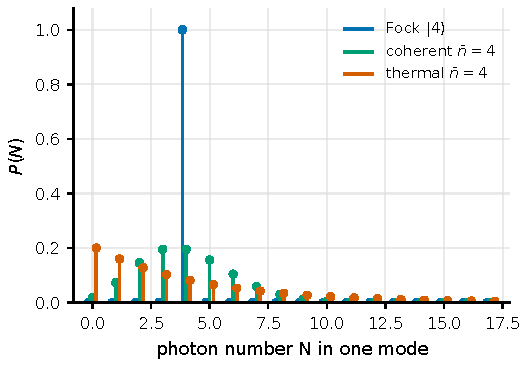
\includegraphics[width=0.82\linewidth]{figures/generated/chapter_03/ch03_state_count_distributions.pdf}
\caption{同一平均光子数附近，数态、相干态和热态给出完全不同的计数分布 \(P(N)\)。数态是一根钉死的竖线（光子数无涨落，\(b_2=1-1/n<1\)）；相干态是泊松分布，宽度约为 \(\sqrt{\bar n}\)（\(b_2=1\)）；热态是几何分布，拖着一条长长的高光子数尾巴（\(b_2=2\)，聚束）。正是这条尾巴，让热光在零延迟处更容易"成对"到达。}
\label{fig:e06-count-distributions}
\end{figure}

图 \ref{fig:e06-count-distributions} 的教益极简：\emph{平均光子数不是全部}。数态没有光子数涨落，相干态有泊松涨落，热态还额外背着一层强度涨落。天文强度干涉利用的，正是热态这最后一层涨落。

\section{压缩态：把量子噪声搬家}
\label{sec:e06-squeezed}

前三种光讲的是"光子数怎么分布"。压缩态（squeezed state）要讲一件不同的事：\emph{量子噪声可以在两个正交的场分量之间重新分配}。它不改变光子成对统计的那套语言，而是回到第 \ref{chap:e04} 章的正交分量（quadrature）图像。

先定义一个相位角 \(\theta\) 上的正交分量算符：
\begin{equation}
  \hat X_\theta=\frac{1}{2}\left(\hat a\,e^{-i\theta}+\hat a^{\dagger}e^{i\theta}\right).
  \label{eq:e06-quadrature}
\end{equation}
\begin{formulaexplain}
\(\hat X_\theta\) 是场沿相位方向 \(\theta\) 的"投影"，是第 \ref{chap:e04} 章位置/动量算符的推广：\(\theta=0\) 给类"位置"分量，\(\theta=\pi/2\) 给类"动量"分量。它无量纲，度量的是场在相空间某个方向上的坐标。
\end{formulaexplain}

逐个交代。\(\hat X_\theta\) 无量纲；\(\theta\) 是我们选定的相空间"观察角度"（弧度）；\(\hat a,\hat a^\dagger\) 是老熟人。取 \(\theta=0\) 得 \(\hat X_0=\tfrac12(\hat a+\hat a^\dagger)\)，正比于第 \ref{chap:e04} 章的位置算符 \(\hat x\)；取 \(\theta=\pi/2\) 得 \(\hat X_{\pi/2}=\tfrac{1}{2i}(\hat a-\hat a^\dagger)\)，正比于动量算符 \(\hat p\)。这两个正交方向就是相空间的"横轴与纵轴"。

关键的量子事实是：\textbf{真空态（以及任何相干态）在每一个方向上的涨落都相等}，方差都是 \(1/4\)。这个基线值不难算，值得当场兑现——它只用到真空的两条性质 \(\hat a|0\rangle=0\) 与对易关系 \([\hat a,\hat a^\dagger]=1\)。真空里 \(\langle\hat X_\theta\rangle=0\)（\(\hat a,\hat a^\dagger\) 的期望都为零），所以方差就等于 \(\langle\hat X_\theta^2\rangle\)。把定义 \eqref{eq:e06-quadrature} 平方展开：
\[
  \hat X_\theta^{2}
  =\frac14\big(\hat a\,e^{-i\theta}+\hat a^\dagger e^{i\theta}\big)^2
  =\frac14\big(\hat a^2 e^{-2i\theta}+\hat a^{\dagger 2}e^{2i\theta}
     +\hat a\hat a^\dagger+\hat a^\dagger\hat a\big).
\]
逐项对真空求期望：含 \(\hat a^2\) 的项因 \(\hat a|0\rangle=0\) 归零；含 \(\hat a^{\dagger2}\) 的项其厄米共轭同样归零；\(\hat a^\dagger\hat a\,|0\rangle=0\)（数算符作用在真空上为零）；只剩 \(\langle 0|\hat a\hat a^\dagger|0\rangle\)，用 \(\hat a\hat a^\dagger=\hat a^\dagger\hat a+[\hat a,\hat a^\dagger]=\hat n+1\) 得 \(\langle0|\hat a\hat a^\dagger|0\rangle=0+1=1\)。于是
\[
  \Delta X_\theta^{2}\big|_{\text{真空}}=\langle\hat X_\theta^2\rangle
  =\frac14\cdot 1=\frac{1}{4}\qquad(\text{对一切 }\theta).
\]
结果和 \(\theta\) 无关，正说明真空在相空间里是一个各向同性的"圆斑"——这也是下一节相空间图像的出发点。海森堡不确定性要求两个正交方向方差之积不小于 \(\tfrac{1}{16}\)，真空恰好取到这个最小值（\(\tfrac14\times\tfrac14=\tfrac1{16}\)）。

压缩态做的事，是把这个圆斑\emph{捏扁}：沿某个方向把方差压到 \(1/4\) 以下，代价是共轭方向的方差被相应抬高。设压缩参数（squeezing parameter）为 \(r\ge0\)，则
\begin{equation}
  \Delta X_{\text{sq}}^{2}=\frac{1}{4}\,e^{-2r},
  \qquad
  \Delta X_{\text{anti}}^{2}=\frac{1}{4}\,e^{+2r}.
  \label{eq:e06-squeeze-var}
\end{equation}
\begin{formulaexplain}
被压缩方向的方差乘上 \(e^{-2r}<1\)（噪声变小），被反压缩方向的方差乘上 \(e^{+2r}>1\)（噪声变大）。\(r\) 越大，一个方向越"扁"、另一个方向越"胖"。
\end{formulaexplain}

这个 \(e^{\mp 2r}\) 的形状来自单模压缩变换：它把相空间沿一个正交方向的振幅尺度乘上 \(e^{-r}\)，方差（尺度的平方）就乘上 \(e^{-2r}\)；共轭方向的尺度乘 \(e^{+r}\)，方差乘 \(e^{+2r}\)。最要紧的是把两个方差乘起来：
\[
  \Delta X_{\text{sq}}^{2}\cdot\Delta X_{\text{anti}}^{2}
  =\frac14 e^{-2r}\cdot\frac14 e^{+2r}
  =\frac{1}{16}\,e^{-2r+2r}
  =\frac{1}{16}.
\]
乘积\emph{仍然}是 \(1/16\)，和真空一模一样！这句话是理解压缩的钥匙：\textbf{压缩没有消灭量子噪声，它只是把噪声从一个方向搬到了另一个方向}——按下葫芦起了瓢，总量守恒。你可以让某个正交分量安静到真空以下，但必须让它的共轭分量吵闹起来做补偿。

实验文献常用分贝（dB）记噪声相对真空的比例：\(10\log_{10}(e^{-2r})\)。例如噪声方差降到真空的十分之一，就是 \(-10\,\text{dB}\)。现代压缩光实验在 \(1064\,\text{nm}\) 附近已能稳定做出 \(10\)–\(15\,\text{dB}\) 的噪声压低，并已用在引力波探测器上把散粒噪声压到标准量子极限以下 \citep{1983Natur.306..141W,2016PhRvL.117k0801V}。

但对天文学要泼一盆冷水：\textbf{普通恒星连续谱并不默认具有压缩}。热态和相干态在每个正交方向上的涨落都不小于真空，谈不上"压扁"。压缩是一种需要非线性光学过程（如参量下转换）精心制备的非经典态，恒星、星云这类自然热源不会自发产生它。我们介绍压缩态，一是为了补全"同一个模式能装哪几种光"的完整图谱，二是因为它在\emph{仪器端}至关重要——未来量子增强的望远镜后端可能用压缩光来突破散粒噪声。但把它当成天体光的默认模型，是一个要避免的误区。

\section{弱热光极限：为超分辨埋下的线}
\label{sec:e06-weak}

最后一节把热态推到天文最常见的角落：\emph{每个模式其实很暗}。第 \ref{chap:e05} 章算过，可见光下恒星的单模占有数 \(\bar n_\nu\sim10^{-2}\ll1\)。在这个弱热光（weak thermal light）极限下，热态会退化成一个特别简单、特别有用的形式。

从几何分布出发，把 \(P(N)\) 在 \(\bar n\ll 1\) 时展开到最低阶。零光子的概率是
\[
  P(0)=\frac{1}{1+\bar n}\simeq 1-\bar n+\mathcal O(\bar n^{2}),
\]
这里用了 \((1+\bar n)^{-1}=1-\bar n+\bar n^2-\cdots\) 的几何级数展开（\(\bar n<1\) 收敛），只保留到一阶。一光子的概率是
\[
  P(1)=\frac{\bar n}{(1+\bar n)^{2}}
  \simeq\bar n\,(1-2\bar n+\cdots)
  \simeq\bar n+\mathcal O(\bar n^{2}).
\]
两光子及以上的概率则是
\[
  P(N\ge 2)=\mathcal O(\bar n^{2}),
\]
因为 \(P(2)=\bar n^2/(1+\bar n)^3\sim\bar n^2\)，是更高阶的小量。也就是说，弱热光里\emph{绝大多数相干时间窗是空的}，偶尔有一个窗里蹦出一个光子，而两个光子同窗则是二阶稀有事件。

把这个层级写成密度矩阵，就得到弱热光的标准记账形式：
\begin{equation}
  \rho\simeq(1-\varepsilon)\,\rho_0+\varepsilon\,\rho_1+\mathcal O(\varepsilon^{2}),
  \qquad
  \varepsilon\equiv\bar n\ll 1,
  \label{eq:e06-weak}
\end{equation}
\begin{formulaexplain}
\(\rho_0=|0\rangle\langle 0|\) 是真空部分（占比 \(1-\varepsilon\)），\(\rho_1=|1\rangle\langle 1|\) 是一光子部分（占比 \(\varepsilon\)），\(\varepsilon=\bar n\) 是单模平均光子数。弱热光就是"大多为空、偶尔一个"的稀疏光子流。
\end{formulaexplain}

逐个交代：\(\rho_0\) 是真空态的密度矩阵，\(\rho_1\) 是单光子态的密度矩阵，小参数 \(\varepsilon=\bar n\) 无量纲，恰好等于上面 \(P(1)\) 的最低阶——所以\emph{把 \(\varepsilon\) 认成"该模式在该时间窗里的平均光子数"是精确的}。式 \eqref{eq:e06-weak} 说的是：光态几乎全是真空，只掺进了一点点单光子成分。这个"一点点"，正是携带天体信息的东西。

为什么要为它专门开一节？因为它是后面\textbf{量子超分辨}（quantum super-resolution）的出发点。既然每个相干时间窗里通常没有光子、偶尔才有一个，那么真正携带天体空间信息的，就是那被探测到的\emph{一光子模式}的空间结构。Tsang、Nair 与 Lu 的弱热光超分辨理论正是从式 \eqref{eq:e06-weak} 这样的展开出发，证明只要能巧妙地测量这一个光子的模式（而不是简单地数强度），就能突破经典的瑞利极限 \citep{2015Optic...2..646T,2016PhRvX...6c1033T}。我们会在第 \ref{chap:e12} 章把这条线接上，讲 SPADE（spatial-mode demultiplexing）如何逼近两颗靠得极近的星的分辨极限。这也和天文事件表天然吻合：零光子的时间窗根本不会被存进文件，留在数据里的，就是那些带时间戳的、稀疏的单光子点击。

\section{相空间图像：把四种光画成一张图}
\label{sec:e06-phasespace}

把这一章收束到一张\emph{看得见}的图上。相空间（phase space）用两个正交分量 \(X\)（横轴）和 \(P\)（纵轴）张成一个平面，把一个模式的量子态画成这个平面上的一团"概率云"——云的中心是平均场，云的胖瘦是涨落。上一节说过，真空和相干态在每个方向的涨落都是 \(1/4\)，所以画出来是一个各向同性的\emph{圆斑}。四种光在这张图上各有各的样子：

\begin{itemize}
  \item \textbf{真空态}：圆斑在原点，半径由 \(1/4\) 的涨落定出。这是所有噪声的"底座"。
  \item \textbf{相干态}：一个\emph{一模一样大小的圆斑}，只是被平移到离原点 \(|\alpha|\) 处。它把真空的圆斑整体搬了个家，形状不变——所以相干态是"移动了的真空"，噪声和真空一样小、一样各向同性。这对应它的 \(b_2=1\)。
  \item \textbf{热态}：一个\emph{中心仍在原点、但更胖的圆}。它没有固定相位（辐角完全随机），又有强度涨落，所以概率云向四面八方摊开，半径随 \(\bar n\) 增大。这个"更胖"，正是热态额外方差 \(\bar n^2\) 的相空间形象，也对应它的 \(b_2=2\)。
  \item \textbf{压缩态}：一个\emph{被压扁的椭圆}。沿被压缩方向窄到真空以下（\(\tfrac14 e^{-2r}\)），沿共轭方向被撑胖（\(\tfrac14 e^{+2r}\)），但椭圆的面积（两个半轴之积对应的方差乘积 \(1/16\)）和圆斑一样——"噪声搬家、面积守恒"在图上就是"圆压成等面积的椭圆"。
\end{itemize}

图 \ref{fig:e06-phase-space} 把相干态、热态、压缩态的这三种"云"并排画了出来。

\begin{figure}[tbp]
\centering
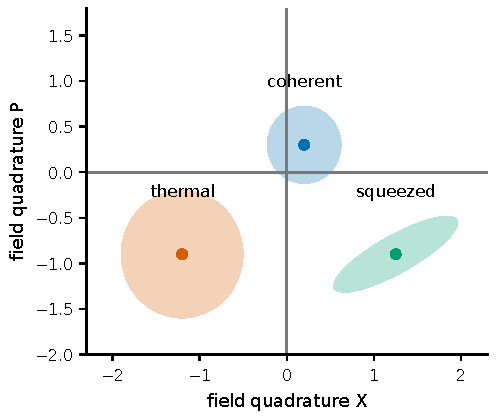
\includegraphics[width=0.72\linewidth]{figures/generated/chapter_03/ch03_phase_space_states.pdf}
\caption{相空间中三类单模光态的涨落形状。相干态是与真空同样大小、只是被平移的圆斑（"移动的真空"）；热态因随机相位和强度涨落而摊成更胖的圆；压缩态把一个正交方向的涨落压到真空以下、同时把共轭方向抬高，成为等面积的椭圆。记住：区分不同光态的，首先是涨落与关联的\emph{形状}，而不只是平均强度。}
\label{fig:e06-phase-space}
\end{figure}

这张相空间图给出一句能带走的话：\emph{不同光态的区别，首先表现为涨落和关联的形状，而不只是平均强度}。同样的亮度，可以是一个安分的圆斑（相干态）、一个躁动的胖圆（热态），或一个被捏扁的椭圆（压缩态）——而正是这些形状，决定了探测器上点击的成对统计。带着这幅图，我们就能进入第 \ref{chap:e07} 章，看这些光态如何在光电探测器上真正变成一串可分析的事件。

\section{本章要点}
\label{sec:e06-summary}

\begin{itemize}
  \item \textbf{尺子：零延迟成对因子} \(b_2=\langle\hat n(\hat n-1)\rangle/\langle\hat n\rangle^2\)。分子用阶乘矩 \(\hat n(\hat n-1)\) 而非 \(\hat n^2\)，因为"同一个光子不能和自己配对"，自配对要扣掉。\(b_2=1\) 是独立泊松基线，\(>1\) 聚束，\(<1\) 反聚束（非经典）。
  \item \textbf{数态 \(|n\rangle\)}：\(P(N)=\delta_{Nn}\)，光子数钉死。\(\langle\hat n\rangle=n\)、\(\langle\hat n(\hat n-1)\rangle=n(n-1)\)，给 \(b_2=1-1/n<1\)。单光子 \(n=1\) 给 \(b_2=0\)，是反聚束的理想极限。
  \item \textbf{相干态 \(|\alpha\rangle\)}：\(\hat a|\alpha\rangle=\alpha|\alpha\rangle\)，\(\bar n=|\alpha|^2\)，计数是泊松分布。逐项求和（砍零项、约阶乘、换元、用指数级数）得 \(\langle N(N-1)\rangle=\bar n^2\)，故 \(b_2=1\)。看到一个光子不改变马上再看到一个的概率。
  \item \textbf{热态 \(\rho_{\text{th}}\)}：几何/玻色分布，\(\langle N\rangle=\bar n\)、\(\operatorname{Var}=\bar n(1+\bar n)\)、\(\langle N(N-1)\rangle=2\bar n^2\)，故 \(b_2=2\)。多出的一倍来自强度涨落（亮时一起多、暗时一起少），这正是 Hanbury Brown--Twiss 聚束的种子。
  \item \textbf{压缩态}：正交分量 \(\hat X_\theta=\tfrac12(\hat a e^{-i\theta}+\hat a^\dagger e^{i\theta})\)，真空方差 \(1/4\)；压缩/反压缩方差 \(\tfrac14 e^{\mp 2r}\)，乘积仍 \(1/16\)——噪声被搬家、不被消灭。普通恒星光不默认压缩，它主要在仪器端有用。
  \item \textbf{弱热光极限}：\(\bar n\ll1\) 时 \(\rho\approx(1-\varepsilon)\rho_0+\varepsilon\rho_1\)，\(\varepsilon=\bar n\)，由几何分布最低阶 \(P(0)\approx1-\bar n\)、\(P(1)\approx\bar n\) 得到。大多数时间窗为空，携带空间信息的是那个被探测到的单光子模式——通往第 \ref{chap:e12} 章超分辨。
  \item \textbf{相空间}：相干态=移动的真空圆斑，热态=更胖的圆，压缩态=等面积的扁椭圆。区分光态的首先是涨落形状，而非平均强度。
\end{itemize}

\medskip
\noindent\textbf{想一想。}
\begin{enumerate}
  \item 把两个独立的单模热光（各自 \(b_2=2\)）非相干地叠加成一个"双模"通道，观测到的成对因子会大于 2、等于 2 还是小于 2？这和第 \ref{chap:e05} 章"多模稀释"的说法一致吗？
  \item 对同一个平均光子数 \(\bar n=10\)，数态、相干态、热态的计数方差各是多少？哪个最"安静"、哪个最"吵"？
  \item 若某个天体源被测得 \(b_2<1\)，能立刻断言它是非经典光源吗？在下结论前，你还需要排除哪些会把 \(b_2\) 拉高或拉低的仪器与混合效应（回顾第 \ref{chap:e05} 章的模式数 \(M\)）？
\end{enumerate}
